% Copyright (c) 2011-2015 by the University of Waikato, Hamilton, NZ.
% This work is made available under the terms of the 
% Creative Commons Attribution-ShareAlike 4.0 license,
% http://creativecommons.org/licenses/by-sa/4.0/.
%
% Version: $Revision$

\documentclass[a4paper]{book}

\usepackage{wrapfig}
\usepackage{graphicx}
\usepackage{hyperref}
\usepackage{multirow}
\usepackage{scalefnt}
\usepackage{tikz}

% watermark -- for draft stage
\usepackage[firstpage]{draftwatermark}
\SetWatermarkLightness{0.9}
\SetWatermarkScale{5}

% Copyright (c) 2009 by the University of Waikato, Hamilton, NZ. 
% This work is made available under the terms of the 
% Creative Commons Attribution-ShareAlike 4.0 license,
% http://creativecommons.org/licenses/by-sa/4.0/.
%
% Version: $Revision: 5479 $

\newenvironment{tight_itemize}{
\begin{itemize}
  \setlength{\itemsep}{1pt}
  \setlength{\parskip}{0pt}
  \setlength{\parsep}{0pt}}{\end{itemize}
}

\newenvironment{tight_enumerate}{
\begin{enumerate}
  \setlength{\itemsep}{1pt}
  \setlength{\parskip}{0pt}
  \setlength{\parsep}{0pt}}{\end{enumerate}
}

% if you just need a simple heading
% Usage:
%   \heading{the text of the heading}
\newcommand{\heading}[1]{
  \vspace{0.3cm} \noindent \textbf{#1} \newline
}

\newcommand{\icon}[1]{\tikz[baseline=-3pt]\node[inner sep=0pt,outer sep=0pt]{\includegraphics[height=1.1em]{#1}};}


\title{
  \textbf{ADAMS} \\
  {\Large \textbf{A}dvanced \textbf{D}ata mining \textbf{A}nd \textbf{M}achine
  learning \textbf{S}ystem} \\
  {\Large Module: adams-moa} \\
  \vspace{1cm}
  
\includegraphics[width=3cm]{images/moa_logo.png} \\
}
\author{
  Albert Bifert \\
  Peter Reutemann
}

\setcounter{secnumdepth}{3}
\setcounter{tocdepth}{3}

\begin{document}

\begin{titlepage}
\maketitle

\thispagestyle{empty}
\center
\begin{table}[b]
	\begin{tabular}{c l l}
		\parbox[c][2cm]{2cm}{\copyright 2011-2015} &
		\parbox[c][2cm]{5cm}{
\includegraphics[width=5cm]{images/coat_of_arms.pdf}} \\
	\end{tabular}
	
\includegraphics[width=12cm]{images/cc.png} \\
\end{table}

\end{titlepage}

\tableofcontents
\listoffigures
%\listoftables

%%%%%%%%%%%%%%%%%%%%%%%%%%%%%%%%%%%
\chapter{Introduction}

\begin{wrapfigure}{r}{0.37\textwidth}
  \vspace{-20pt}
  \centering
  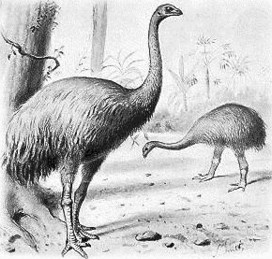
\includegraphics[width=0.35\textwidth]{images/moa-bird.png}
  \caption{MOA, the (extinct) New Zealand bird.}
  \label{moa-bird}
\end{wrapfigure}  

MOA (``Massive Online Analysis'', \cite{moa}) is a framework for data stream mining. It 
includes a collection of machine learning algorithms (classification, 
regression, and clustering) and tools for evaluation. Related to the WEKA 
project, MOA is also written in Java, while scaling to more demanding problems.

\chapter{Flow}
If you are familiar with the WEKA actors in ADAMS, then you won't have any
problems getting up to speed with using MOA in the flow. The following sections
explain the various actors in more detail.

\section{Data sources}
Since MOA uses the WEKA data structures as backend, you can basically use any
actor that outputs \texttt{weka.core.Instance} tokens as source for the other
MOA actors. MOA also comes with a range of stream generators for artificial
data (or ARFF-file based ones), which you can make use of the 
\textit{MOAStream} source. Figure \ref{moa-stream-flow} shows a 
flow\footnote{adams-moa-datastream.flow} that generates some artificial data
with a stream generator and displays it (see Figure \ref{moa-stream-output}).

\begin{figure}[htb]
  \centering
  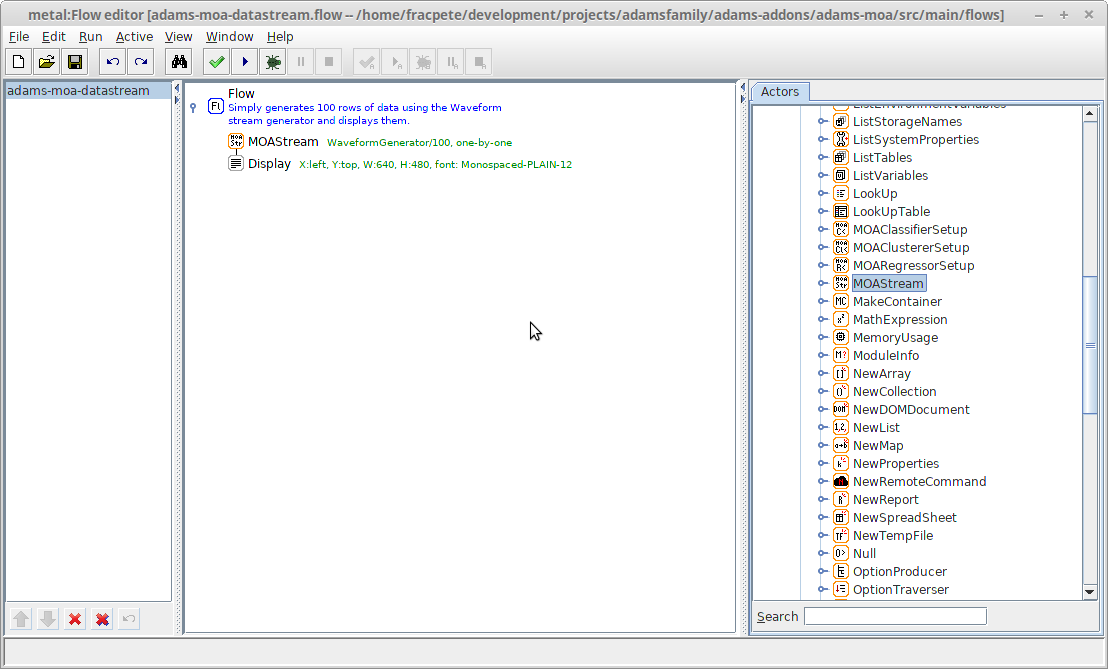
\includegraphics[width=12.0cm]{images/moa-stream-flow.png}
  \caption{Flow for generating and displaying artificial data.}
  \label{moa-stream-flow}
\end{figure}

\begin{figure}[htb]
  \centering
  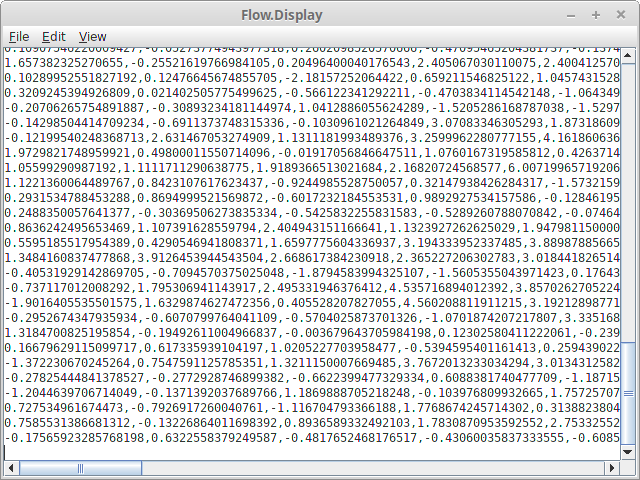
\includegraphics[width=12.0cm]{images/moa-stream-output.png}
  \caption{The generated data.}
  \label{moa-stream-output}
\end{figure}

\clearpage
\newpage
\section{Classification}
Classification in the flow work very similar to ones for WEKA.
But instead of performing cross-validation or train/test splits, you use a
special stream evaluator which performs an evaluation every X instances that
come through. The transformer performing the evaluation is 
\textit{MOAClassifierEvaluation}. It references a callable classifier of type 
\textit{MOAClassifierSetup} to evaluate on the data stream and also what type of MOA 
evaluation you want to perform.
Figures \ref{moa-classifier-flow} and \ref{moa-classifier-output} show a 
flow\footnote{adams-moa-classifier\_evaluation.flow} 
and its associated output (kappa and percentage correct). The classifier is 
being evaluated every 100 instances of the 10,000 that the stream generator 
outputs.

\begin{figure}[htb]
  \centering
  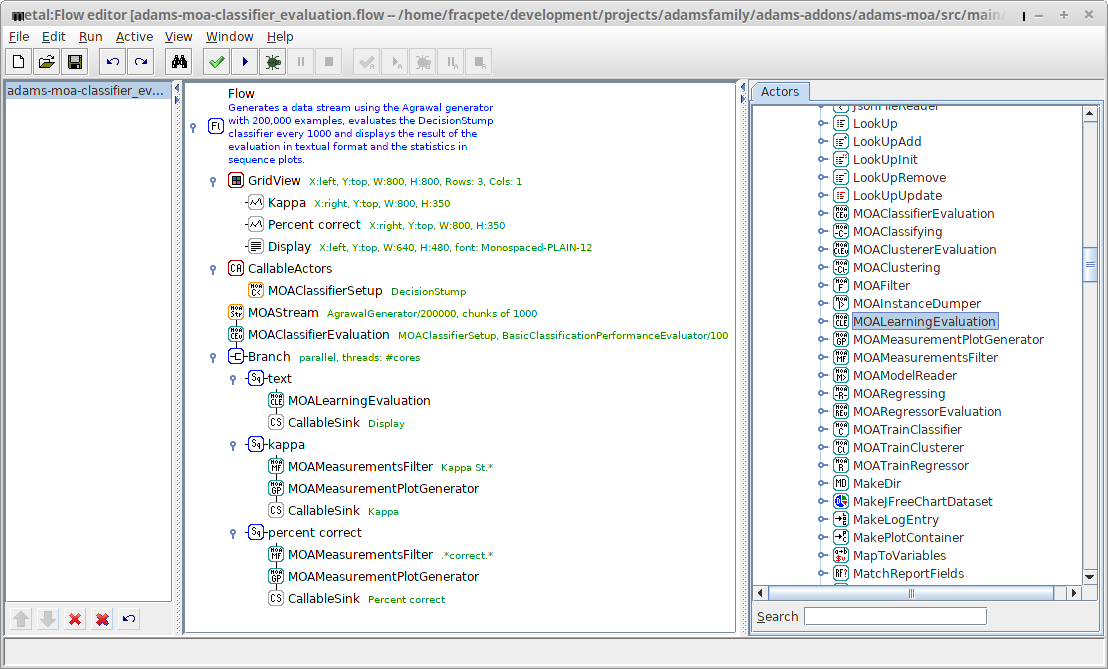
\includegraphics[width=12.0cm]{images/moa-classifier-flow.png}
  \caption{Flow for evaluating a classifier on a stream.}
  \label{moa-classifier-flow}
\end{figure}

\begin{figure}[htb]
  \centering
  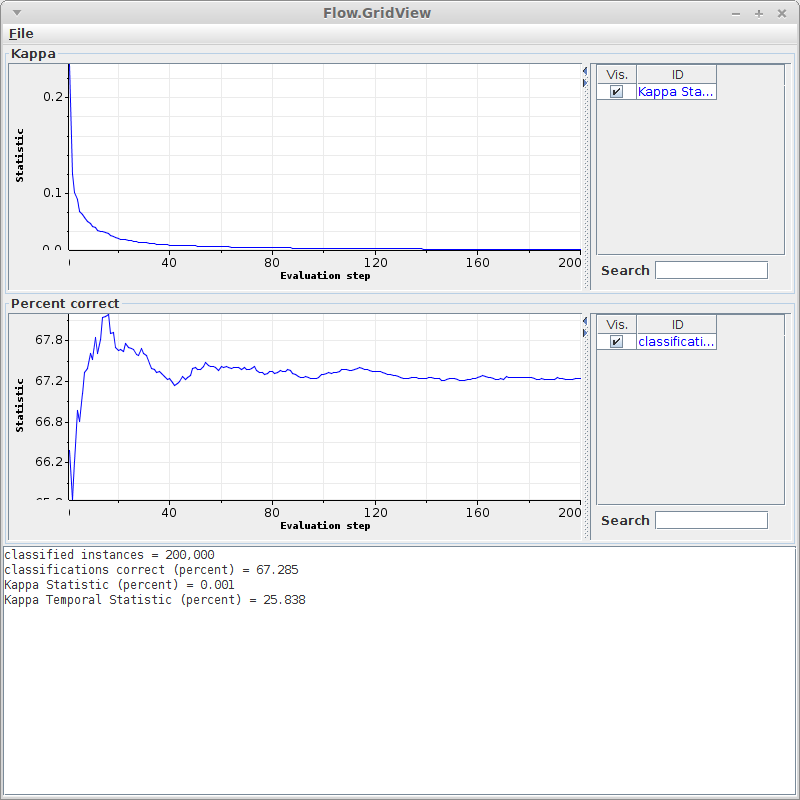
\includegraphics[width=12.0cm]{images/moa-classifier-output.png}
  \caption{The evaluation result.}
  \label{moa-classifier-output}
\end{figure}

\clearpage
Just like with WEKA, you can also use a serialized classifier to classify 
incoming data. First, you need to train and serialize a classifier. How this
is done, is shown in the flow\footnote{adams-moa-serialize\_classifier\_model.flow} 
in Figure \ref{moa-serialize-classifier}.
This flow uses the \textit{MOAModelWriter} sink to save the trained classifier
to a file. Then, you can use this serialized model (e.g., loading it with the 
\textit{MOAModelReader}) in conjunction with the 
\textit{MOAClassifying} transformer to make predictions on the incoming data.
Figures \ref{moa-classifying-flow} and \ref{moa-classifying-output} show the
flow\footnote{adams-moa-classifying\_with\_model.flow} and the predicted
class distributions for the incoming data.

There are some transformers that help you turning the evaluation object that
the \textit{MOAClassifierEvaluation} outputs into useful output:
\begin{tight_itemize}
	\item \textit{MOALearningEvaluation} -- generates a string represenation of
	the evaluation object
	\item \textit{MOAMeasurementsFilter} -- picks the measurements from the
	evaluation that match the regular expression (matching sense can be inverted).
	\item \textit{MOAMeasurementPlotGenerator} -- turns a measurement into a
	plot container that can be displayed in the \textit{SequencePlotter} sink.
\end{tight_itemize}

\begin{figure}[htb]
  \centering
  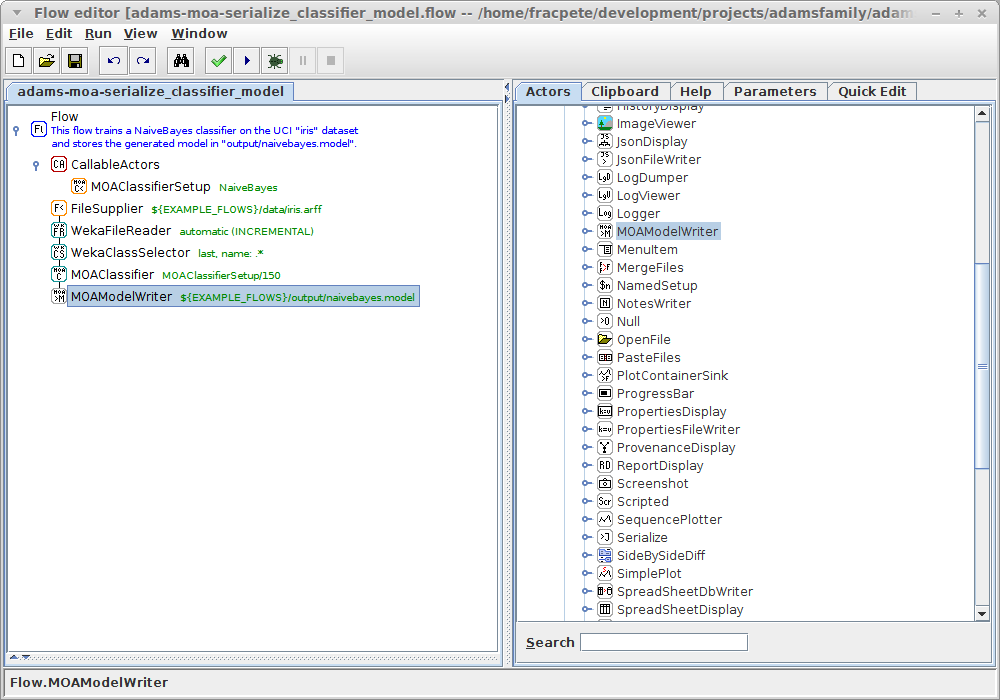
\includegraphics[width=12.0cm]{images/moa-serialize-classifier.png}
  \caption{Flow for serializing a trained classifier.}
  \label{moa-serialize-classifier}
\end{figure}

\begin{figure}[htb]
  \centering
  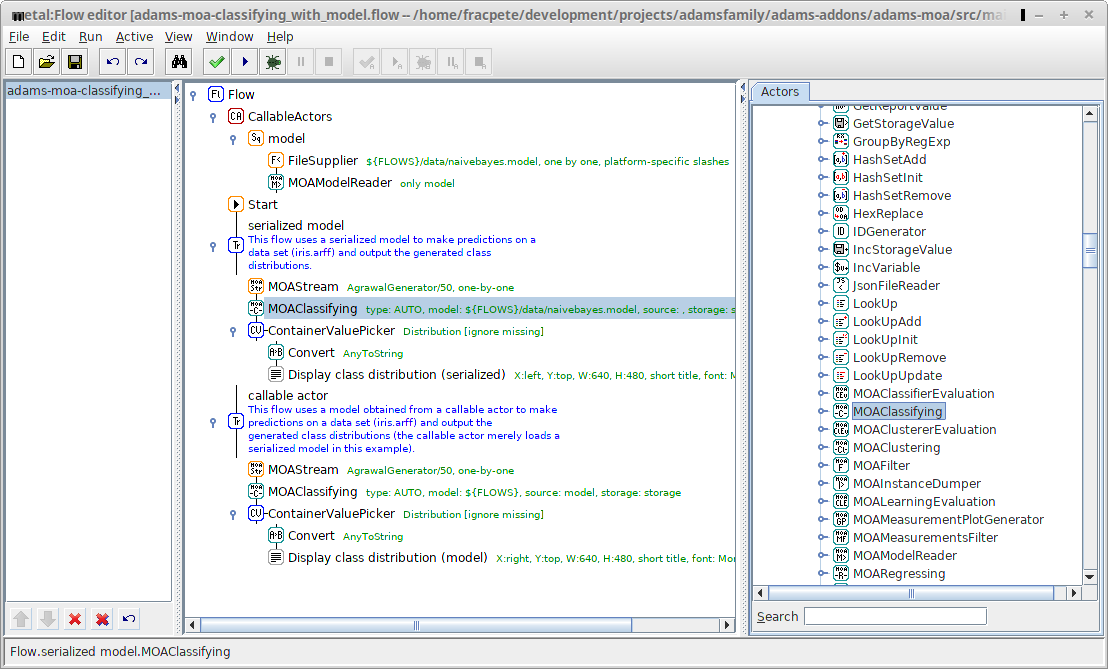
\includegraphics[width=12.0cm]{images/moa-classifying-flow.png}
  \caption{Flow for classifying data using a pre-built model.}
  \label{moa-classifying-flow}
\end{figure}

\begin{figure}[htb]
  \centering
  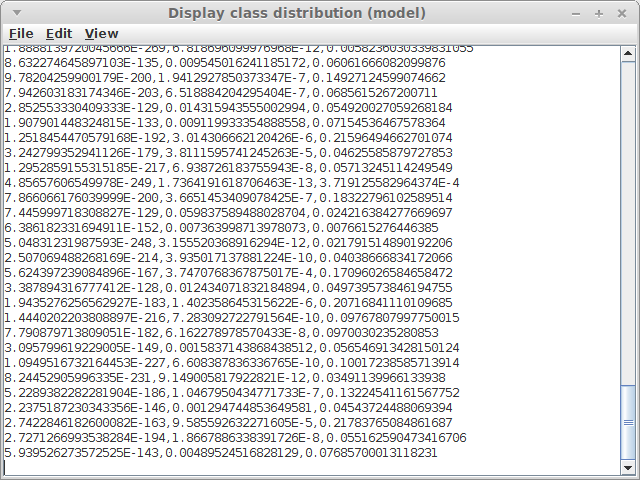
\includegraphics[width=12.0cm]{images/moa-classifying-output.png}
  \caption{The classification result.}
  \label{moa-classifying-output}
\end{figure}

\clearpage
\newpage
\section{Regression}
Regression is very similar to classification with the corresponding actors
below:
\begin{tight_itemize}
  \item \textit{source.MOARegressorSetup} -- outputs a regressor object.
  \item \textit{transformer.MOARegressing} -- makes predictions on the incoming
  data\footnote{adams-moa-regressing\_with\_model.flow}.
  \item \textit{transformer.MOARegressorEvaluation} -- evaluates a regressor on
  a data stream\footnote{adams-moa-regressor\_evaluation.flow}.
  \item \textit{transformer.MOATrainRegressor} -- builds a regressor model on
  a data stream.
\end{tight_itemize}

\clearpage
\newpage
\section{Clustering}
At the moment, only cluster visualization is available in the flow\footnote{adams-moa-cluster\_visualization.flow}:
\begin{tight_itemize}
  \item \textit{MOAClustererSetup} -- source for defining cluster algorithm setups
  \item \textit{MOAClusterVisualization} -- sink that visualizes clusterings
\end{tight_itemize}

\begin{figure}[htb]
  \centering
  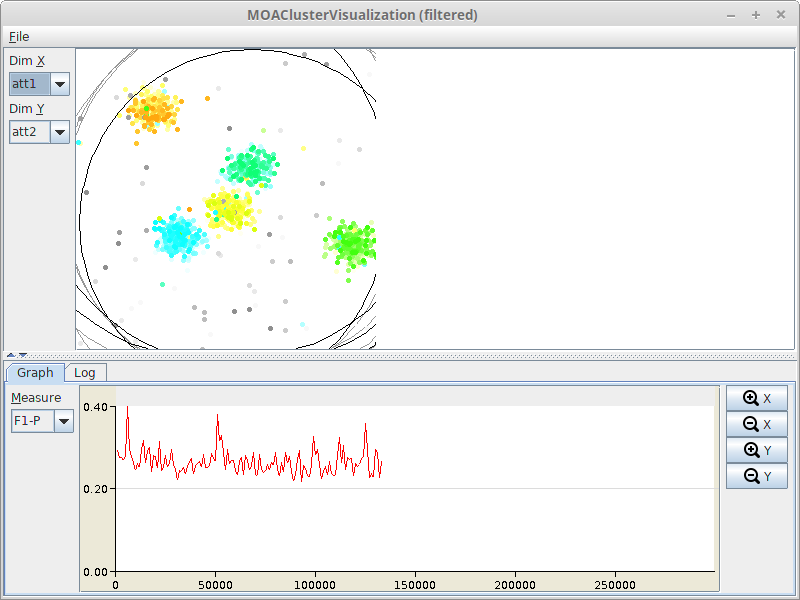
\includegraphics[width=12.0cm]{images/moa-cluster_visualization.png}
  \caption{Cluster visualization.}
  \label{moa-cluster_visualization}
\end{figure}

\clearpage
\newpage
\section{Filtering}
Even though there is no filtering support in MOA at the time of writing, it is
possible using WEKA's stream filters to filter data streams in MOA.
You can use the \textit{WekaStreamFilter} transformer to apply one of WEKA's
stream filters to the stream of \textit{weka.core.Instance} objects passing
through.

In Figure \ref{moa-stream-filtering_flow} you can see a flow\footnote{adams-moa-filtering.flow} 
that generates a data stream using the \textit{RandomRBFGenerator} class. It
outputs a stream with 40 attributes and 4 class labels. This flow applies
the \textit{DownSample} filter (only uses every nth attribute) to the stream
and plots the classifier performance, percentage correct and kappa, in a graph
(see Figure \ref{moa-stream-filtering_output}). Three plots are generated: evaluation
on the full attribute range, down-sampled with using only every 2nd and 4th
attribute.

\begin{figure}[htb]
  \centering
  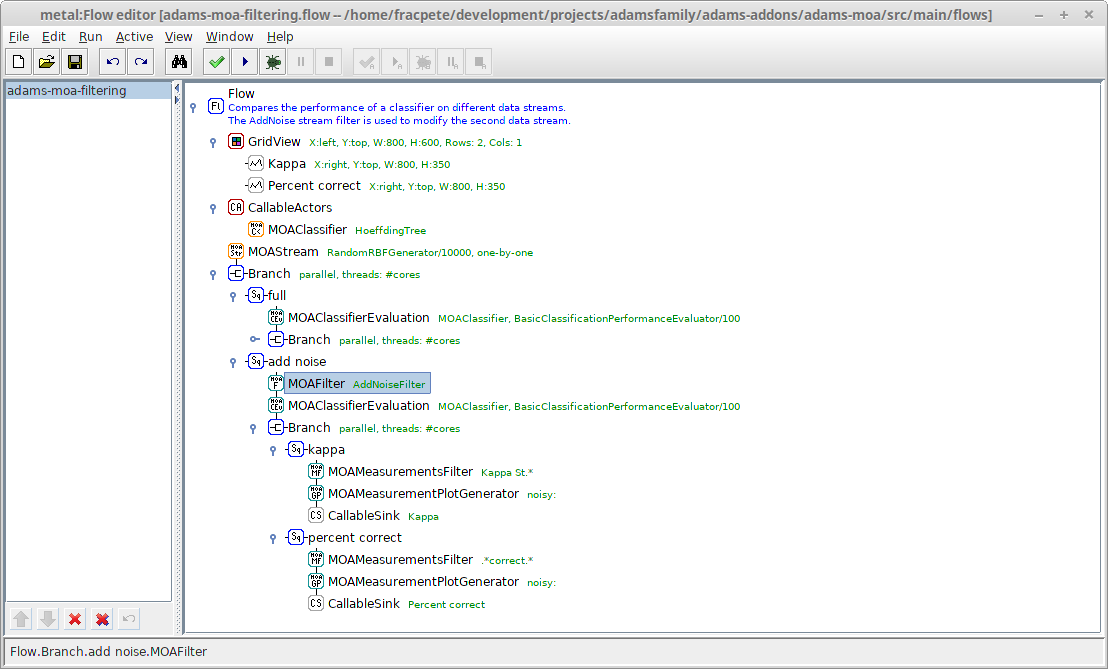
\includegraphics[width=12.0cm]{images/moa-stream-filtering_flow.png}
  \caption{Filtering data streams.}
  \label{moa-stream-filtering_flow}
\end{figure}

\begin{figure}[htb]
  \centering
  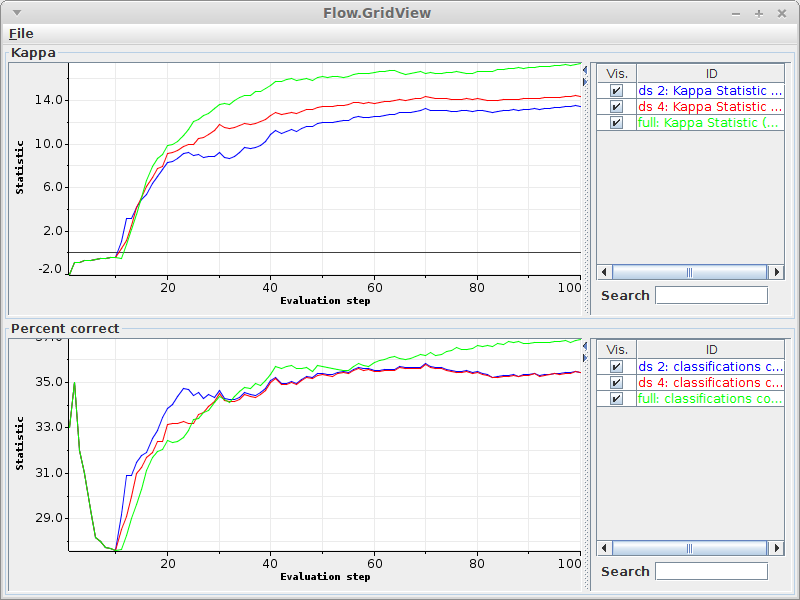
\includegraphics[width=12.0cm]{images/moa-stream-filtering_output.png}
  \caption{Comparisong of streams, filtered and unfiltered.}
  \label{moa-stream-filtering_output}
\end{figure}

\clearpage
\newpage
\section{Provenance}
Just like with WEKA, provenance is supported by MOA's actors as well.
In Figure \ref{provenance-flow} you can see a 
flow\footnote{adams-moa-classifier\_provenance.flow} that will display the
provenance information that the tokens accumulated, from generation through 
to evaluation. Figure \ref{provenance-output} then shows the visualization
of the provenance trace.

\begin{figure}[htb]
  \centering
  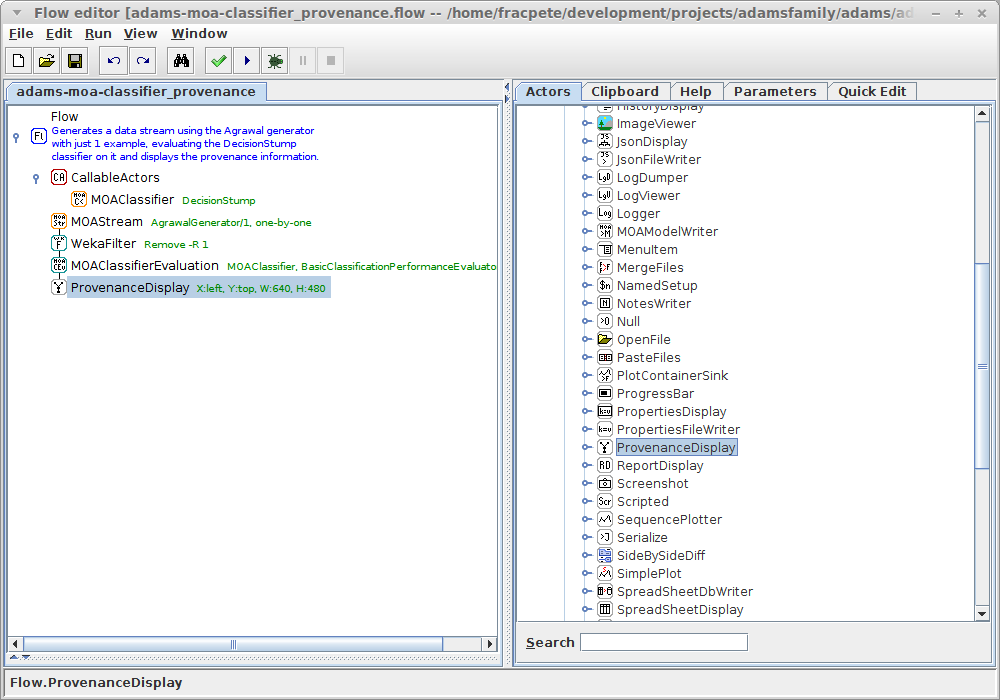
\includegraphics[width=12.0cm]{images/provenance-flow.png}
  \caption{Flow for displaying provenance information.}
  \label{provenance-flow}
\end{figure}

\begin{figure}[htb]
  \centering
  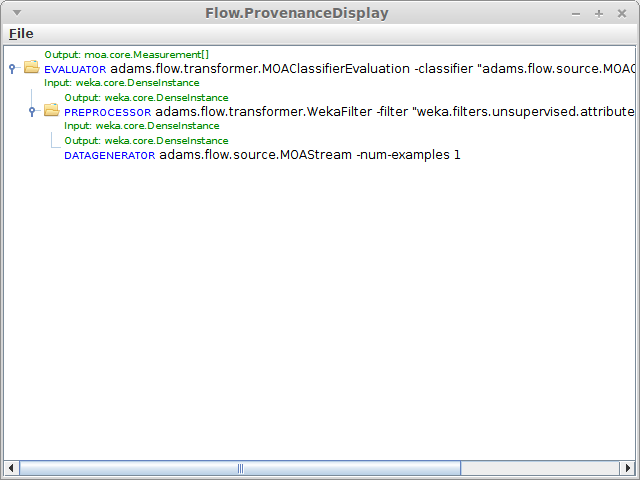
\includegraphics[width=12.0cm]{images/provenance-output.png}
  \caption{The generated provenance trace.}
  \label{provenance-output}
\end{figure}

\chapter{Tools}
The main interface for MOA is available from within ADAMS as well. You can
find it under the \textit{MOA} menu. Figure \ref{moa-gui} shows a screenshot
of the user interface in action.
\begin{figure}[htb]
  \centering
  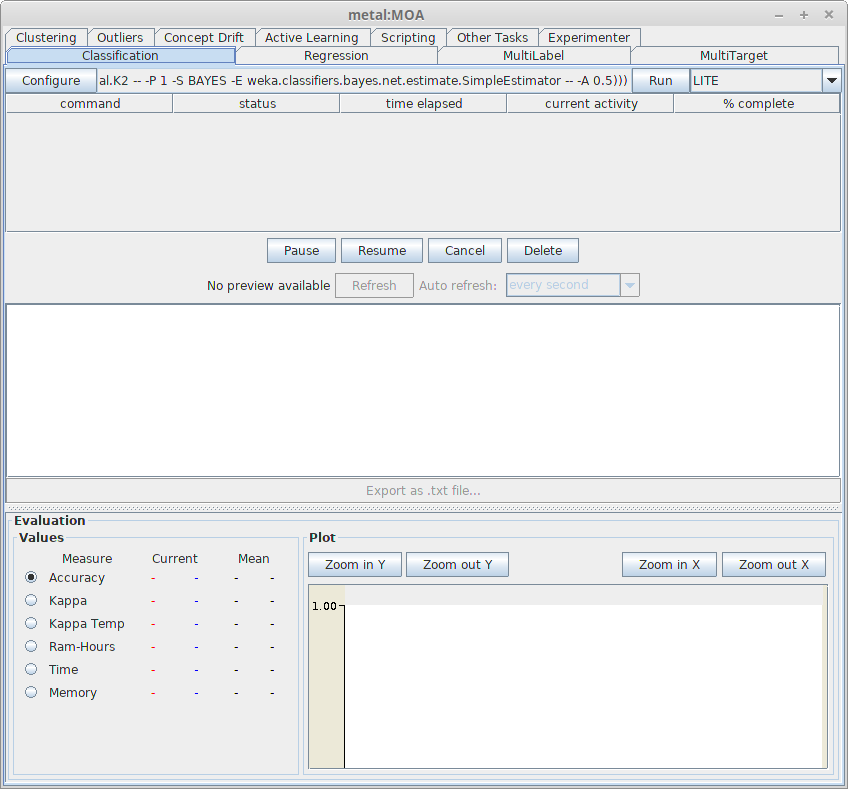
\includegraphics[width=12.0cm]{images/moa-gui.png}
  \caption{The main MOA interface.}
  \label{moa-gui}
\end{figure}


%%%%%%%%%%%%%%%%%%%%%%%%%%%%%%%%%%%
% Copyright (c) 2009-2012 by the University of Waikato, Hamilton, NZ. 
% This work is made available under the terms of the 
% Creative Commons Attribution-ShareAlike 4.0 license,
% http://creativecommons.org/licenses/by-sa/4.0/.
%
% Version: $Revision$

\begin{thebibliography}{999}
	% to make the bibliography appear in the TOC
	\addcontentsline{toc}{chapter}{Bibliography}

    % references
	\bibitem{adams}
		\textit{ADAMS} -- Advanced Data mining and Machine learning System \\
		\url{https://adams.cms.waikato.ac.nz/}{}
		
	\bibitem{heatmap}
		\textit{Heat map} -- WikiPedia article \\
		\url{http://en.wikipedia.org/wiki/Heat_map}{}

\end{thebibliography}


\end{document}
